
%!TEX root = handout.tex


\section{OpenMS - Getting started}

%%%%%%%%%%%%%%%%%%%%%%%%%%%%%%%%%%%%%%%%%%%%%%%%%%%%%%%%%%%%%%%%%%%%%%%%%%%%%%%%

Before we get started we will install OpenMS and KNIME using the installers provided on the USB stick. Please choose the directory that matches your operating system and execute the installer. Note that these steps are not necessary if you use one of our laptops.

For example for Windows you call
\begin{itemize}
\item the OpenMS installer: \directory{Windows / OpenMS-2.0\_Win64\_setup.exe}
\item the KNIME installer: \directory{Windows / OpenMS-2.0-prerequisites-installer.exe} \\ and \directory{Windows / KNIME\ 2.12.0\ Installer\ (64bit).exe}
\end{itemize}

on Mac you call
\begin{itemize}
\item the OpenMS installer: \directory{Mac / OpenMS-2.0.0\_setup.dmg}
\item the KNIME installer: \directory{Mac / knime\_2.12.0.macosx.cocoa.x86\_64.dmg}
\end{itemize}

and follow the instructions.

\subsection{Data conversion}
\label{Data_Conversion}

Each MS instrument vendor has one or more formats for storing the acquired data. Converting these data into an open format (preferably mzML) is the very first step when you want to work with open-source mass spectrometry software. A freely available conversion tool is ProteoWizard. The OpenMS installation package for Windows automatically installs ProteoWizard, so you do not need to download and install it separately.

Please note that due to restrictions from the instrument vendors, file format conversion for most formats is only possible on Windows systems, so exporting from the acquisition PC connected to the instrument is usually the most convenient option.
All files used in this tutorial have already been converted to mzML by us, so you do not need to do it yourself.

%%%%%%%%%%%%%%%%%%%%%%%%%%%%%%%%%%%%%%%%%%%%%%%%%%%%%%%%%%%%%%%%%%%%%%%%%%%%%%%%

\subsection{Data visualization using \OPENMSTOOL{TOPPView}}
\label{Data_Visualization}

Visualizing the data is the first step in quality control, an essential tool in understanding the data, and of course an essential step in pipeline development.
OpenMS provides a convenient viewer for some of the data: \OPENMSTOOL{TOPPView}.

\begin{figure}
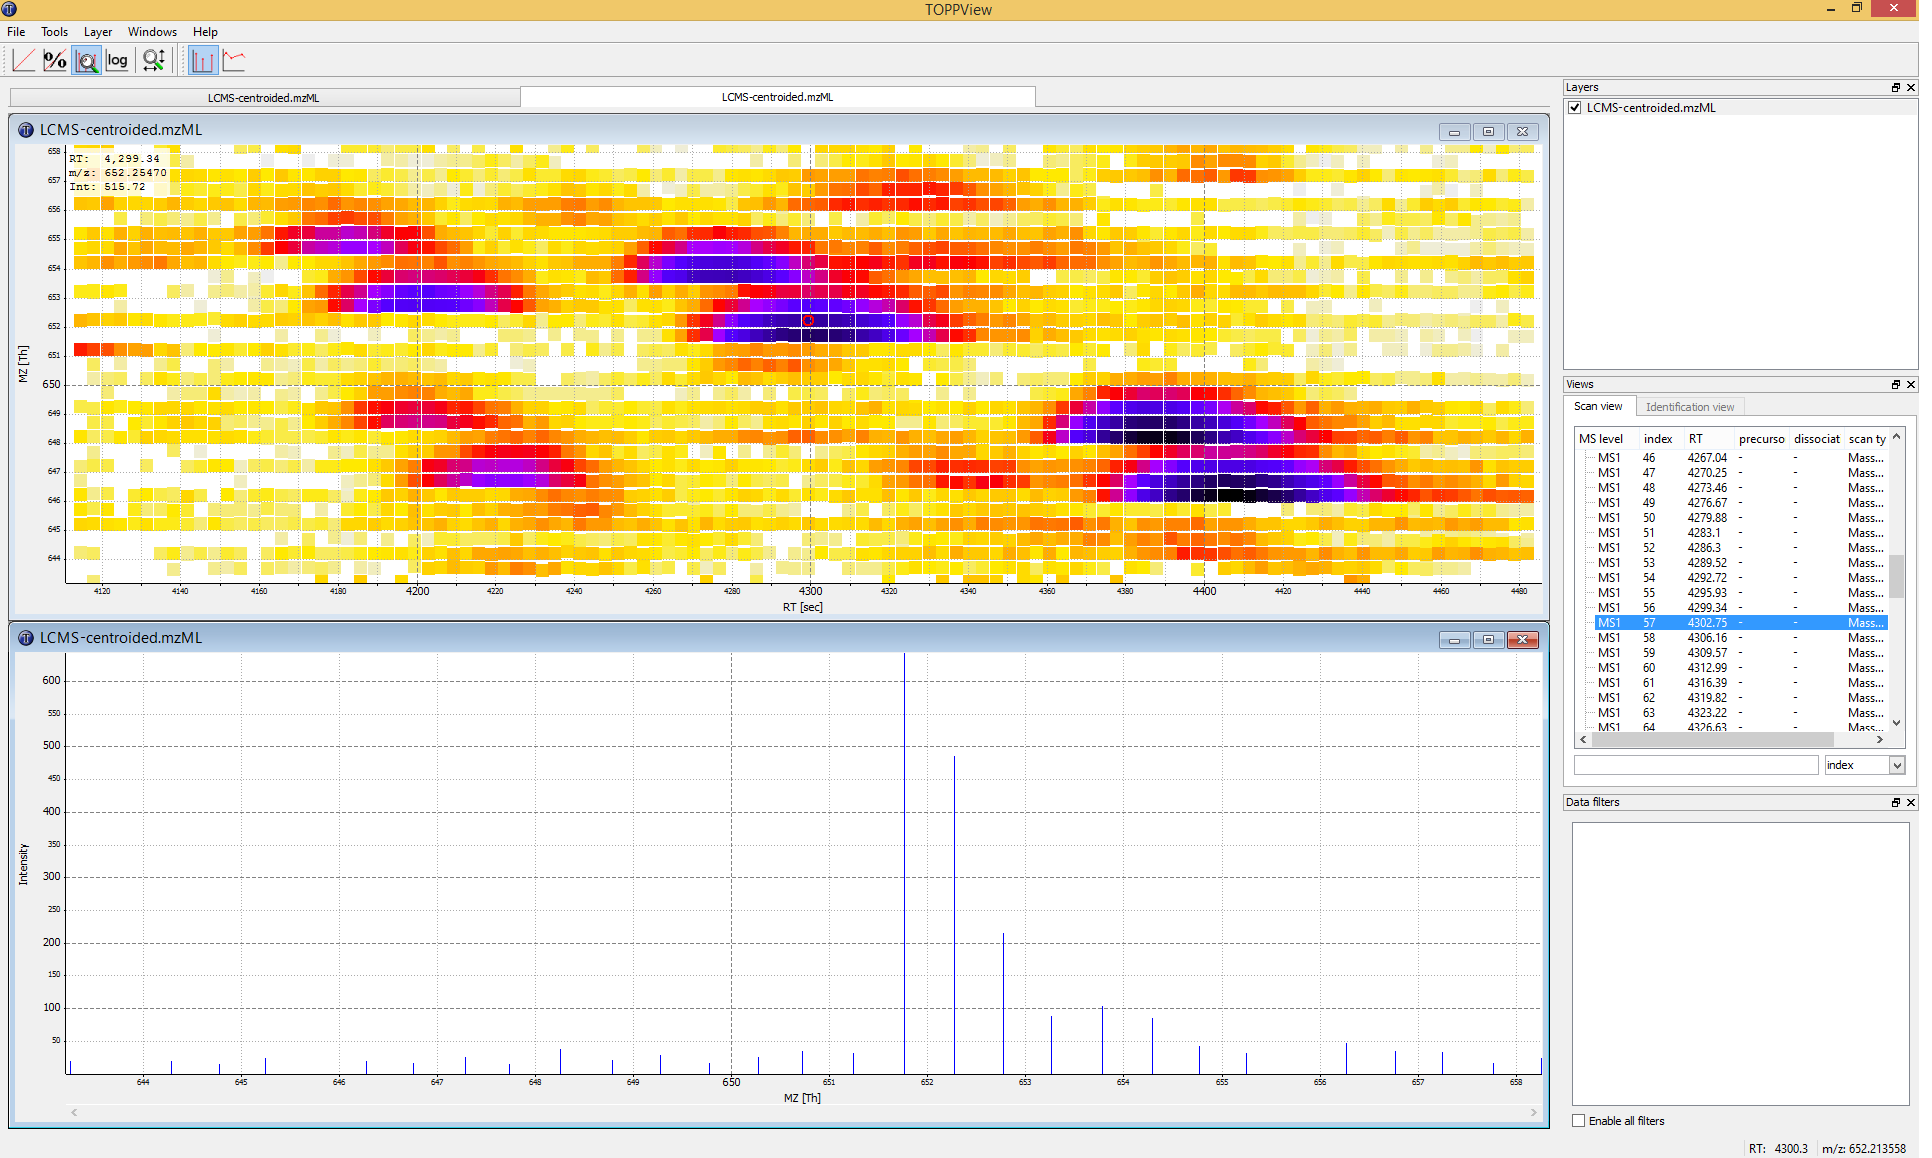
\includegraphics[width=\textwidth]{graphics/introduction/TOPPView.png}
\caption{TOPPView, the graphical application for viewing mass spectra and analysis results. Top window shows a small region of a peak map. In this 2D representation of the measured spectra, signals of eluting peptides are colored according to the raw peak intensities. The lower window displays an extracted spectrum (=scan) from the peak map. On the right side, the list of spectra can be browsed.}
\label{fig:toppview}
\end{figure}

We will guide you through some of the basic features of \OPENMSTOOL{TOPPView}. Please familiarize yourself with the key controls and visualization methods.
We will make use of these later throughout the tutorial. Let's start with a first look at one of the files of our tutorial data set:

\begin{itemize}
\item Start \OPENMSTOOL{TOPPView} (see Start-Menu or Applications on MacOS)
\item Go to \menu{File > Open File}, navigate to the directory where you copied the contents of the USB stick to,
      and select
      \directory{Example\_Data / Introduction / datasets / small / velos005614.mzML}
      . This file contains a reduced LC-MS map (only a selected RT and m/z range
      was extracted using the TOPP tool \OPENMSTOOL{FileFilter}) of a label-free measurement of the human platelet proteome recorded on an Orbitrap velos.
      The other two mzML files contain technical replicates of this experiment.
      First, we want to obtain a global view on the whole LC-MS map - the default option \textit{Map view 2D} is the correct one and we can click the \menu{Ok} button. 
\item Play around.
\item Three basic modes allow you to interact with the displayed data: scrolling, zooming and measuring:
    \begin{itemize}
    \item Scroll mode
        \begin{itemize}
        \item Is activated by default (though each loaded spectra file is displayed zoomed out first, so you do not need to scroll).
        \item Allows you to browse your data by moving around in RT and m/z range.
        \item When zoomed in, to scroll the spectra map, click-drag on the current view.
        \item Arrow keys can be used to scroll the view as well.
        \end{itemize}
    \item Zoom mode
        \begin{itemize}
        \item Zooming into the data: either mark an area in the current view with your mouse while holding the left mouse
              button plus the \keys{\ctrl} key to zoom to this area
              or use your mouse wheel to zoom in and out.
        \item All previous zoom levels are stored in a zoom history. The zoom history can be traversed using
              \keys[,]{\ctrl,+} or \keys[,]{\ctrl,-} or the mouse wheel (scroll up and down).
        \item Pressing the Backspace key zooms out to show the full LC-MS map (and also resets the zoom history).
        \end{itemize}
    \item Measure mode
        \begin{itemize}
        \item It is activated using the \keys{\shift} key.
        \item Press the left mouse button down while a peak is selected and drag the mouse to
        			another peak to measure the distance between peaks.
        \item This mode is implemented in the 1D and 2D mode only.
        \end{itemize}
    \end{itemize}
\item Right click on your 2D map and select \menu{Switch to 3D view} and examine your
			data in 3D mode
\item Go back to the 2D view. In 2D mode, visualize your data in different normalization modes, use linear, percentage and log-view (icons on the upper left tool bar).
\note{On \textit{Apple OS X}, due to a bug in one of the external libraries used by OpenMS, you will see a small window of the 3D mode when switching to 2D. Close the 3D tab in order to get rid of it.}
\item In \OPENMSTOOL{TOPPView} you can also execute TOPP tools. Go to
			\menu{Tools > Apply tool (whole layer)} and choose a TOPP tool (e.g., FileInfo) and
			inspect the results.
\end{itemize}
